\documentclass[12pt,letterpaper]{article}
\usepackage{graphicx,textcomp}
\usepackage{natbib}
\usepackage{setspace}
\usepackage{fullpage}
\usepackage{color}
\usepackage[reqno]{amsmath}
\usepackage{amsthm}
\usepackage{fancyvrb}
\usepackage{amssymb,enumerate}
\usepackage[all]{xy}
\usepackage{endnotes}
\usepackage{lscape}
\newtheorem{com}{Comment}
\usepackage{float}
\usepackage{hyperref}
\newtheorem{lem} {Lemma}
\newtheorem{prop}{Proposition}
\newtheorem{thm}{Theorem}
\newtheorem{defn}{Definition}
\newtheorem{cor}{Corollary}
\newtheorem{obs}{Observation}
\usepackage[compact]{titlesec}
\usepackage{dcolumn}
\usepackage{tikz}
\usetikzlibrary{arrows}
\usepackage{multirow}
\usepackage{xcolor}
\newcolumntype{.}{D{.}{.}{-1}}
\newcolumntype{d}[1]{D{.}{.}{#1}}
\definecolor{light-gray}{gray}{0.65}
\usepackage{url}
\usepackage{listings}
\usepackage{color}

\definecolor{codegreen}{rgb}{0,0.6,0}
\definecolor{codegray}{rgb}{0.5,0.5,0.5}
\definecolor{codepurple}{rgb}{0.58,0,0.82}
\definecolor{backcolour}{rgb}{0.95,0.95,0.92}

\lstdefinestyle{mystyle}{
	backgroundcolor=\color{backcolour},   
	commentstyle=\color{codegreen},
	keywordstyle=\color{magenta},
	numberstyle=\tiny\color{codegray},
	stringstyle=\color{codepurple},
	basicstyle=\footnotesize,
	breakatwhitespace=false,         
	breaklines=true,                 
	captionpos=b,                    
	keepspaces=true,                 
	numbers=left,                    
	numbersep=5pt,                  
	showspaces=false,                
	showstringspaces=false,
	showtabs=false,                  
	tabsize=2
}
\lstset{style=mystyle}
\newcommand{\Sref}[1]{Section~\ref{#1}}
\newtheorem{hyp}{Hypothesis}

\title{Problem Set 2}
\date{Due: October 16, 2022}
\author{Applied Stats/Quant Methods 1}

\begin{document}
	\maketitle
	\section*{Instructions}
\begin{itemize}
	\item Please show your work! You may lose points by simply writing in the answer. If the problem requires you to execute commands in \texttt{R}, please include the code you used to get your answers. Please also include the \texttt{.R} file that contains your code. If you are not sure if work needs to be shown for a particular problem, please ask.
	\item Your homework should be submitted electronically on GitHub.
	\item This problem set is due before 23:59 on Sunday October 16, 2022. No late assignments will be accepted.
	\item Total available points for this homework is 80.
\end{itemize}

	
	\vspace{.5cm}
	\section*{Question 1 (40 points): Political Science}
		\vspace{.25cm}
	The following table was created using the data from a study run in a major Latin American city.\footnote{Fried, Lagunes, and Venkataramani (2010). ``Corruption and Inequality at the Crossroad: A Multimethod Study of Bribery and Discrimination in Latin America. \textit{Latin American Research Review}. 45 (1): 76-97.} As part of the experimental treatment in the study, one employee of the research team was chosen to make illegal left turns across traffic to draw the attention of the police officers on shift. Two employee drivers were upper class, two were lower class drivers, and the identity of the driver was randomly assigned per encounter. The researchers were interested in whether officers were more or less likely to solicit a bribe from drivers depending on their class (officers use phrases like, ``We can solve this the easy way'' to draw a bribe). The table below shows the resulting data.

\newpage
\begin{table}[h!]
	\centering
	\begin{tabular}{l | c c c }
		& Not Stopped & Bribe requested & Stopped/given warning \\
		\\[-1.8ex] 
		\hline \\[-1.8ex]
		Upper class & 14 & 6 & 7 \\
		Lower class & 7 & 7 & 1 \\
		\hline
	\end{tabular}
\end{table}

\begin{enumerate}
	
	\item [(a)]
	Calculate the $\chi^2$ test statistic by hand/manually (even better if you can do "by hand" in \texttt{R}).\\
	\vspace{7cm}
	Step 1: Load and Process The Data:\\ 
	\lstinputlisting[language=R, firstline=3, lastline=8]{PS2.R}
	Step 2: Calculate the expected frequency of each cell\\
	\lstinputlisting[language=R, firstline=18, lastline=34]{PS2.R}
	Expected Frequency Upper Class is not stopped 13.5\\
	Expected Frequency Upper Class is bribe requested: 8.36\\
	Expected Frequency Upper Class Stopped/Given warning: 5.14\\
	Expected Frequency Lower Class Not Stopped: 7.5\\
	Expected Frequency Lower Class bribe Requested: 4.64 \\
	Expected Frequency Lower Class Stopped/Given warning: 2.86\\
	Step 3: Calculate the sum of X-square/Test Statistics
	\lstinputlisting[language=R, firstline=44, lastline=45]{PS2.R}
	The sum of X-square/Test Statistics is 3.80.
	
	
	\item [(b)]
	Now calculate the p-value from the test statistic you just created (in \texttt{R}).\footnote{Remember frequency should be $>$ 5 for all cells, but let's calculate the p-value here anyway.}  What do you conclude if $\alpha = 0.1$?\\
	Calculate the degree of freedom\\
	\lstinputlisting[language=R, firstline=48, lastline=49]{PS2.R}
	The degree of freedom is 2.
	The Chi square value with degree of freedom 2, alpha = 0.1 is 4.61.	The test statistics 3.8 $<$ 4.61. The obtained chi-square value did not exceed the critical value of 4.61. Therefore, we cannot reject the null hypothesis that soliciting a bribe by police or not is independent from the class of driver.
	
	
	or
	\lstinputlisting[language=R, firstline=64, lastline=64]{PS2.R}
	p-value is 0.15, which is larger than 0.1. Therefore, we cannot reject the null hypothesis that soliciting a bribe by police or not is independent from the class of driver.
	\newpage
	\item [(c)] Calculate the standardized residuals for each cell and put them in the table below.
	\vspace{1cm}
	\lstinputlisting[language=R, firstline=70, lastline=86]{PS2.R}
	
	
	\begin{table}[h]
		\centering
		\begin{tabular}{l | c c c }
			& Not Stopped & Bribe requested & Stopped/given warning \\
			\\[-1.8ex] 
			\hline \\[-1.8ex]
			Upper class  & 0.1361 & -0.8162 & 0.8204 \\
			\\
			Lower class & -0.1826 & 1.0956  & -1.0998  \\
			
		\end{tabular}
	\end{table}
	
	
	\vspace{7cm}
	\item [(d)] How might the standardized residuals help you interpret the results?  \\
	 The absolute values of standard residuals in all cells are smaller than 2, we can therefore informally conclude that we cannot reject the null hypothesis that the two variables, drivers' class and police's bribing behaviour, are independent. In the cells of upper class not stopped and lower class not stopped, the absolute values of standard residuals are closer to 0, which indicate there is a stronger evidence that the drivers' class and they are not stopped by police are independent from each other. 
	
	
\end{enumerate}
\newpage

\section*{Question 2 (40 points): Economics}
Chattopadhyay and Duflo were interested in whether women promote different policies than men.\footnote{Chattopadhyay and Duflo. (2004). ``Women as Policy Makers: Evidence from a Randomized Policy Experiment in India. \textit{Econometrica}. 72 (5), 1409-1443.} Answering this question with observational data is pretty difficult due to potential confounding problems (e.g. the districts that choose female politicians are likely to systematically differ in other aspects too). Hence, they exploit a randomized policy experiment in India, where since the mid-1990s, $\frac{1}{3}$ of village council heads have been randomly reserved for women. A subset of the data from West Bengal can be found at the following link: \url{https://raw.githubusercontent.com/kosukeimai/qss/master/PREDICTION/women.csv}\\

\noindent Each observation in the data set represents a village and there are two villages associated with one GP (i.e. a level of government is called "GP"). Figure~\ref{fig:women_desc} below shows the names and descriptions of the variables in the dataset. The authors hypothesize that female politicians are more likely to support policies female voters want. Researchers found that more women complain about the quality of drinking water than men. You need to estimate the effect of the reservation policy on the number of new or repaired drinking water facilities in the villages.
\vspace{.5cm}
\begin{figure}[h!]
	\caption{\footnotesize{Names and description of variables from Chattopadhyay and Duflo (2004).}}
	\vspace{.5cm}
	\centering
	\label{fig:women_desc}
	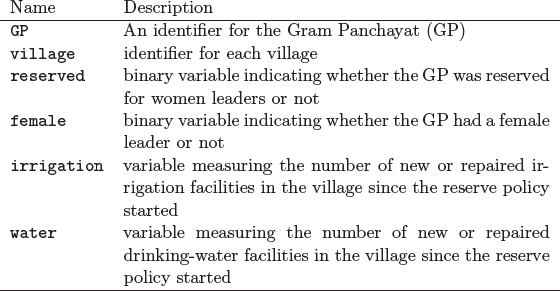
\includegraphics[width=1.1\textwidth]{women_desc.png}
\end{figure}		

\newpage
\begin{enumerate}
	\item [(a)] State a null and alternative (two-tailed) hypothesis. \\
	Null Hypothesis: There is no correlation between Gender of GP leaders and the likelihood of the number of new or repaired drinking water facilities in the villages. \\
	\vspace{6cm}
	\item [(b)] Run a bivariate regression to test this hypothesis in \texttt{R} (include your code!).
	Step 1: load data\\
	\lstinputlisting[language=R, firstline=103, lastline=103]{PS2.R}
	Step 2: run a bivariate regression
	\lstinputlisting[language=R, firstline=112, lastline=117]{PS2.R}	
	\href{file:///C:/Users/Caesar/Documents/GitHub/StatsI_Fall2022/problemSets/PS02/My_Answers/Reg_Gen_Wat.html}{\includegraphics[height=.99\textheight]{Reg_Gen_Wat.html}}
	
	\item [(c)] Interpret the coefficient estimate for reservation policy.\\ 
	The p-value of the coefficient of female is 0.0197, which is lower than 0.05.
	Therefore, we can reject the null hypothesis that there is no correlation between the existence of reservation policy and the number of new or repaired drinking water facilities in the villages at the 95 per cent level.\\ 
	The coefficient of reserved is 9.252, which indicates that when there is a reservation policy in place, we expect to see an average difference by 9.252 higher in the number of new or repaired drinking water facilities in the villages.
\end{enumerate}

\end{document}
